\chapter{Introduction and Background}

\section{The Spaghetti Syndrome and its Implications - the need for a Wireless Vital Signs Monitoring System}

Modern surgeries are challenging working environments involving a combination of complex devices, computers and humans working under stressful and time critical conditions. However, to date there are far too many wired devices communication between machines, monitoring patient physiological conditions and still requiring considerable attention by experts for monitoring and decision making.

In an era where surgery is ubiquitous, an ever increasing number of devices are attached to critically ill patients, multiplying the number of wires and tubes connected to the patient which results in a net resembling a plate of spaghetti; hence, the coinage of the term the Spaghetti Syndrome \cite{imhoff2004spaghetti}. This conundrum has been present in the context of critical care, anaesthesia, and operating theatres for almost three decades with the advent of new technological advances in medicine \cite{cesarano1979spaghetti}. This issue clearly illustrates the need for a system which is not physically connected to avoid possible harm and injury to both the surgeons and patients in the operating theatre. 

The presence of wires in the surgery room introduces the possibility of increased surgery duration due to tripping hazards. More severe trips could lead to further surgical complications, due to wire disconnections which results in inaccurate readings of vital signs. Consequently, a possible overdose or underdose of anaesthetic agents could follow, leading to patient injury, and in the worst case scenario, the demise of the patient. Indirectly, wires in the operating theatre increase the rate of mortality during surgeries. 

One possible course of action to rectify this problem is to remove cables connected to patients by replacing the medium of transmission from a wire to electromagnetic waves. In recent years, multiple research projects have been carried out with the aim to embed vital sign sensors with wireless technology to separate patients from cables \cite{rosenthal2003new}.  

Nevertheless, most advances in this area of wireless device development is limited to the context of medical centres and not operating theatres.  

\section{Benefits of a Wireless Implementation}

Having a wireless version of current vital signs monitoring systems will bring additional benefits to 


Ease of use - convenience
Less risk of injury
Faster surgery - smaller delay due to obstruction from wires
Safer
Better working environment for doctors

\section{Overview of the Project}

This  paper will  consider the  process and challenges of  developing a fully integrated wireless vital signs monitoring system for vital signs specifically for anaesthetic parameters such as electrocardiography (ECG), photoplethysmography (PPG), electroencephalography (EEG), blood pressure, and blood temperature. The  front end of the project encompasses the collection and processing of raw data from different sensors including the visualisation and presentation of vital signs information,  according  to some specified performance criterion. The back end of the project involves the wireless transmission and reception of the processed information to a fixed output display and possibly, a secure database. 

The aim of this project is to make as many patient monitoring, measuring devices as fully wireless so enabling more freedom of movement for both patients, nurses, and medical staff. What makes this first task challenging is that the wireless network (WA) system must be safe, secure and as reliable as current wired systems. Once completed, we envisage a new program in the development of pervasive wireless network resources for anesthetists and surgical practice in general. In these cases being hands-free, being able to access information, direct activities by simple movement, gestures adds to more efficient and clean surgical practice. \\

The project involves two parts: 

\begin{enumerate}
	\item programming hardware nodes to collect wireless sensor data using Android, and 
	
	\item software application development to visualize the data in real-time. The project also involves estimating missing data and inferring suitable information to medical professionals. The project requires developing a mobile app and also a data analysis platform.
\end{enumerate}


\section{Anaesthetic Parameters for Patient Monitoring}

Countless operations are conducted on a daily basis which requires patients to be under general anaesthesia. To ensure the patient's optimal safety when under anaesthesia, it is necessary to consistently monitor certain parameters to ensure that they remain within a specified range which is considered to be safe or normal. Based on Atlee's Complications in Anesthesia \cite{atlee2006complications}, monitoring of anaesthetic admisnistration reduces the probability of anaesthetic overdose or underdose. 

Complications associated with an improper dosage of anaesthesia could arise such as coma, brain damage, nerve damage, or possibly death, if real-time observations of vital signs are not conducted. The risk of such issues occuring during surgery could be reduced significantly if a feedback system were implemented for the amount of anaesthetics administered to the patient. Such parameters have been stipulated by ANZCA. 

\subsection{Theory of Electrocardiography}

The electrocardiogram (ECG) refers to the recording of the "differences in electrical potential generated by the heart" using electrodes which are placed on the surface of the skin \cite{noble1990electrocardiography}. Both the action potentials generated by individual cells and sequence of activation affect the signal registered during electrocardiography \cite{noble1990electrocardiography}. Other factors which alter the final signal include "the position of the heart within the body, the nature of the intervening tissue, and the distance to the recording electrode" \cite{noble1990electrocardiography}. Despite the many factors which can possibly contribute a change to the electrocardiogram, it is still possible to deduce with high accuracy the state of the heart from the surface ECG due to "the careful correlation of electrocardiographic patterns with observed anatomic, pathologic, and physiologic data" \cite{noble1990electrocardiography}. 


\begin{figure}[H]
	\centering
	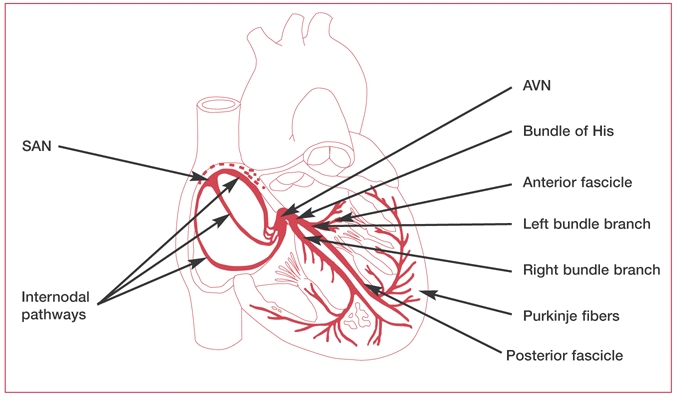
\includegraphics[width=0.7\linewidth]{ch3f3.jpg}
	\caption{The Cardiac Depolarization Route. AVN: Atrioventricular Node; SAN: Sinoatrial Node. \cite{hall2015guyton}}
	\label{cardiacdepolarization}
\end{figure}

\begin{figure}[H]
	\centering
	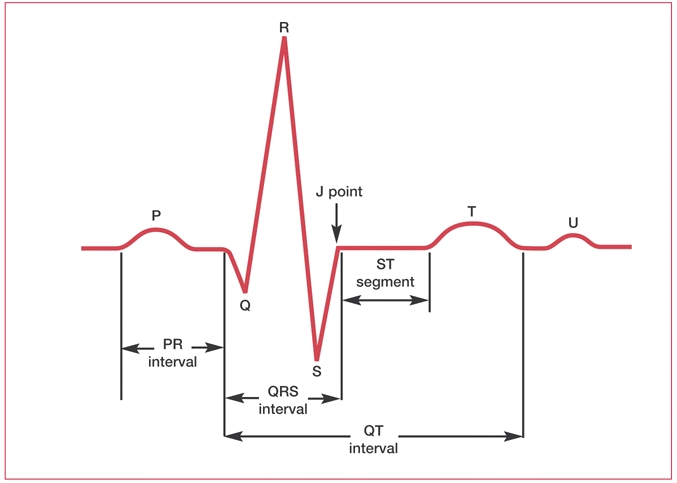
\includegraphics[width=0.7\linewidth]{ch3f4.jpg}
	\caption{The Basic Pattern of Electrical Activity across the Heart \cite{ashley2004conquering}}
	\label{ecgpattern}
\end{figure}

Figure \ref{ecgpattern} shows a graphical representation of a typical electrocardiograph trace of the electrical signals from the heart. 

The basic ECG pattern is correlated as follows: 

\begin{itemize}
	\item "Electrical activity towards a lead causes an upward deflection" \cite{ashley2004conquering}
	\item "Electrical activity away from a lead causes a downward deflection" \cite{ashley2004conquering} 
	\item "Depolarization and repolarization deflections occur in opposite directions" \cite{ashley2004conquering} 
\end{itemize}  

Ashley and Niebauer (2004) (p.g. 19) \cite{ashley2004conquering} succinctly explains the types of waves and intervals of the ECG trace, (which mainly comprises of three different waves, namely P, QRS complex, and T): 

\blockquote{
"The {\bf P wave} is a small deflection wave that represents atrial depolarization. 

The {\bf PR interval} is the time between the first deflection of the P wave and the first deflection of the QRS complex. 

The three waves of the {\bf QRS complex} represent ventricular depolarization. For the inexperienced, one of the most confusing aspects of ECG reading is the labeling of these waves. The rule is: if the wave immediately after the P wave is an upward deflection, it is an R wave; if it is a downward deflection, it is a Q wave:

\begin{itemize}
	\item small {\bf Q waves} correspond to depolarization of the interventricular septum. Q waves can also relate to breathing and are generally small and thin. They can also signal an old myocardial infarction (in which case they are big and wide)
	\item the {\bf R wave} reflects depolarization of the main mass of the ventricles – hence it is the largest wave
	\item the {\bf S wave} signifies the final depolarization of the ventricles, at the base of the heart 
\end{itemize}

The {\bf ST segment}, which is also known as the ST interval, is the time between the end of the QRS complex and the start of the T wave. It reflects the period of zero potential between ventricular depolarization and repolarization. 

{\bf T waves} represent ventricular repolarization (atrial repolarization is obscured by the large QRS complex)." }


\subsection{Theory of Electroencephalography}

\subsection{Theory of Photoplethysmography}

\subsection{Theory of Blood Pressure}

\subsection{Theory of Blood Temperature}
